\chapter{Design moderner Blockchiffren}
Blockchiffre: wenn Klar- und Chiffretext aus Blöcke einer bestimmten Länge bestehen (meist 64 oder 128 Bit) \\
Prinzipien bei Blockchiffren
\begin{itemize}
	\item \textbf{Nicht Empfohlen:} \textit{Security by Inctricacy}, Sicherheit durch Komplexität des Verfahrens
	\item \textbf{Empfohlen:} Systematische Aufbau der Chiffre \texttt{+} Öffentlichkeit des Verfahrens (Kerckhoff'sche Prinzip)
\end{itemize}

Bei symmetrischen Verfahren sollte es keinen besseren Angriff als wie Brute-Force geben. Ciphertext-Only aussichtslos, Chosen-/Known-Plaintext teilweise bekannt. \\
\textbf{Zufallsorakel:} kein erkennbarer Zusammenhang zwischen Eingabe und Ausgabe.

Claude Shannon Forderungen:
\begin{itemize}
	\item \textbf{Konfusion:} Zusammenhang zwischen Klartext und Chiffretext nicht erkennbar machen, um die Ableitung des Schlüssels zu erschweren.
	\item \textbf{Diffusion:} Jedes Bit des Klartextes/Schlüssels beeinflusst möglichst viele Bits des Chiffretexts
	\item \textbf{Nebenforderungen:} effiziente (arbeitsspeicher-, zeit- und stromsparende) Umsetzbarkeit in Software und Hardware, daher einfache Operationen wie XOR, Bitshifts
\end{itemize}

\textbf{Bitpermutationen} sind in Hardware sehr einfach umzusetzen (Hardwarebahnen), in Software jedoch schwieriger. \\
Art und Reihenfolge soll nicht vom Schlüssel oder Klartext abhängen, da dies Seitenkanalangriffe ermöglicht.

Erreichen der Ziele:
\begin{itemize}
	\item \textbf{iterierte Ausführung gleichartiger Runden}: Rundenschlüssel, abgeleitet vom Hauptschlüssel
	\item \textbf{Permutationen} für \textbf{Diffusion}
	\item \textbf{Substitutionen (S-Boxen)} für \textbf{Konfusion}
\end{itemize}

\section{Data Encryption Standard (DES)}
Jahr 1977 unter Beteiligung NSA. Anwendungen: Bankkarten

Einfache Operationen, besonders gute Hardwareimplementierung, Software langsamer.

Klartext- und Chiffretext sind 64 Bit Blöcke, enthält jedoch 8 Prüfbits $\rightarrow$ \textbf{56 Bit Schlüssel}. ($2^{56} = 7 \cdot 10^{16}$)

\textbf{Feistel-Chiffre mit 16 Runden:} Ver- und Entschlüsseln ist gleich.

\textbf{konstante S-Boxen} und \textbf{konstante Permutationen}. S-Boxen wurden auf Sicherheit untersucht und haben die Eigenschaft, dass bei Veränderung eines Eingangbits mindestens 2 Ausgangsbit verändert werden.

Schlüssel mit XOR, da schnell.

\subsection{Schlüsselraum}
Da die effektive Schlüssellänge nur 56 Bit ist, war damals ein Brute-Force Angriff (z.B. durch NSA) erreichbar gewesen. RSA Brute-Force: alle Schlüssel durchprobieren bis sinnvoller Klartext herauskommt, man muss natürlich wissen, was Verschlüsselt wurde (Format, Inhalt Sprache, Codierung,...). Daher ist normaler DES \textbf{nicht mehr sicher}.

\subsection{Blockgröße}
Nachrichten werden in 64 Bit Blöcken unterteilt, ähnlich zu einer Monoalphabetische Substitution mit 64 Bit Blöcke $\rightarrow$ Häufigkeitsanalyse?
\begin{itemize}
	\item Bei gleichgekommen Klartexten, wiederholt sich ein Block nach $2^64$ 64 Bit Blöcke $\rightarrow$ 140 Mio TB, also Nein
	\item Jedoch ist ein 64 Bit Block 8 ASCII Zeichen. Aber trotzdem nein
\end{itemize}

\textbf{Schlüssellänge} beeinflusst Aufwand von Brute Force. \\
\textbf{Blockgröße} beeinflusst Aufwand von Häufigkeitsanalyse. \\
DES ist prinzipiell sicher, aber wegen 56 Bit Schlüssel einfach zu knacken.

\section{Triple-DES, 3DES, DESede}
Das DES prinzipiell, vom Design keine Schwastellen bekannt sind, verwendet man ihn 3x hintereinander um das Problem der Schlüssellänge zu beheben.

Warum nicht 2x? Wegen \textbf{Meet-in-the-Middle Angriff}
\begin{figure}[H]
	\centering
	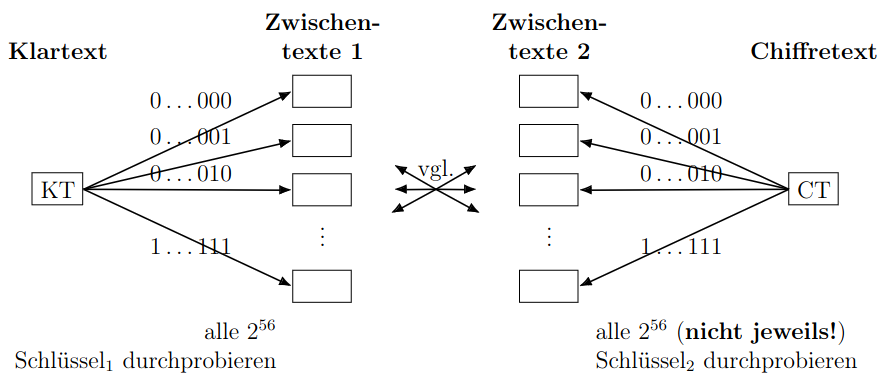
\includegraphics[width=1.0\linewidth]{figures/3des_mitm.png}
	\caption{3DES Meet-in-the-Middle Angriff}
\end{figure}
Ausgang: Kown-Plaintext Angriff, Klartext-Chiffretext-Paar. Es wird der Klartext mit allen $2^{56}$ Schlüsseln verschlüsselt und mit allen $2^{56}$ der Chiffretext entschlüsselt und miteinander verglichen. Bei einer Übereinstimmung ist der Schlüssel bekannt. Man muss nur $2^{56}$ + $2^{56}$ = $2^{57}$ Ver- und Entschlüsselungen durchführen $\rightarrow$ effektiv 57 Bit Schlüssellänge.

Deshalb wendet man DES 3-mal an: $DES_{K1}(DES_{K2}(DES_{K1}(m)))$
Dadurch muss man $2^{112}$ + $2^{56}$ = $2^{112}$ Ver- und Entschlüsselungen durchführen. Meet-in-the-Middle Angriff ist immer noch möglich aber enorm aufwendiger.

Da jedoch DES in Software langsam ist, wegen Speicherbedarf, Strombedarfs,... erhöht man nicht die Rundenzahl, sondern Verwendet andere Verschlüsselungen wie Blowfish, AES,...

\section{Advanced Encryption Standard (AES)}
1997 kam es zu einer Ausschreibung für einen DES-Nachfolger. AES ist gut Ressourcenverbrauch und Leistung in Hard- und Software. AES ist kein Feistel-Chiffre sonder ein \textbf{SP-Netzwerk (Substitution-Permutation)}, deshalb verläuft die Entschlüsselung komplett anders (Erfinder müssen beachten dass die Entschlüsselung auch Effizient ist)

Schlüssellänge: 128, 192 oder 256 Bit \\
Abhängig davon ob 10, 12 oder 14 Runden 128-Bit Blöcker, mit 4 x 4 Byte Matrizen. Eine Runde:
\begin{enumerate}
	\item \textbf{SubBytes:} S-Box Substitutionen (Resistent gegenüber linearer und differentieller Kryptoanalyse)
	\item \textbf{ShiftRows:} Einträge je Zeile werden 0, 1, 2, 3 Einträge nach links rotiert. (Zahlen aus selben Spalten in verschiedenen Spalten)
	\item \textbf{MixColumn:} Zahlen in einer Spalte werden vermischt (lineare Operationen)
	\item \textbf{AddRoundKey:} Rundenschlüssel mit XOR verknüpft
\end{enumerate}

AES wird verwendet in:
\begin{itemize}
	\item WPA2 (WLAN)
	\item KeePass
	\item LTE
\end{itemize}